\documentclass[twoside]{book}

% Packages required by doxygen
\usepackage{fixltx2e}
\usepackage{calc}
\usepackage{doxygen}
\usepackage[export]{adjustbox} % also loads graphicx
\usepackage{graphicx}
\usepackage[utf8]{inputenc}
\usepackage{makeidx}
\usepackage{multicol}
\usepackage{multirow}
\PassOptionsToPackage{warn}{textcomp}
\usepackage{textcomp}
\usepackage[nointegrals]{wasysym}
\usepackage[table]{xcolor}

% Font selection
\usepackage[T1]{fontenc}
\usepackage[scaled=.90]{helvet}
\usepackage{courier}
\usepackage{amssymb}
\usepackage{sectsty}
\renewcommand{\familydefault}{\sfdefault}
\allsectionsfont{%
  \fontseries{bc}\selectfont%
  \color{darkgray}%
}
\renewcommand{\DoxyLabelFont}{%
  \fontseries{bc}\selectfont%
  \color{darkgray}%
}
\newcommand{\+}{\discretionary{\mbox{\scriptsize$\hookleftarrow$}}{}{}}

% Page & text layout
\usepackage{geometry}
\geometry{%
  a4paper,%
  top=2.5cm,%
  bottom=2.5cm,%
  left=2.5cm,%
  right=2.5cm%
}
\tolerance=750
\hfuzz=15pt
\hbadness=750
\setlength{\emergencystretch}{15pt}
\setlength{\parindent}{0cm}
\setlength{\parskip}{3ex plus 2ex minus 2ex}
\makeatletter
\renewcommand{\paragraph}{%
  \@startsection{paragraph}{4}{0ex}{-1.0ex}{1.0ex}{%
    \normalfont\normalsize\bfseries\SS@parafont%
  }%
}
\renewcommand{\subparagraph}{%
  \@startsection{subparagraph}{5}{0ex}{-1.0ex}{1.0ex}{%
    \normalfont\normalsize\bfseries\SS@subparafont%
  }%
}
\makeatother

% Headers & footers
\usepackage{fancyhdr}
\pagestyle{fancyplain}
\fancyhead[LE]{\fancyplain{}{\bfseries\thepage}}
\fancyhead[CE]{\fancyplain{}{}}
\fancyhead[RE]{\fancyplain{}{\bfseries\leftmark}}
\fancyhead[LO]{\fancyplain{}{\bfseries\rightmark}}
\fancyhead[CO]{\fancyplain{}{}}
\fancyhead[RO]{\fancyplain{}{\bfseries\thepage}}
\fancyfoot[LE]{\fancyplain{}{}}
\fancyfoot[CE]{\fancyplain{}{}}
\fancyfoot[RE]{\fancyplain{}{\bfseries\scriptsize Generated by Doxygen }}
\fancyfoot[LO]{\fancyplain{}{\bfseries\scriptsize Generated by Doxygen }}
\fancyfoot[CO]{\fancyplain{}{}}
\fancyfoot[RO]{\fancyplain{}{}}
\renewcommand{\footrulewidth}{0.4pt}
\renewcommand{\chaptermark}[1]{%
  \markboth{#1}{}%
}
\renewcommand{\sectionmark}[1]{%
  \markright{\thesection\ #1}%
}

% Indices & bibliography
\usepackage{natbib}
\usepackage[titles]{tocloft}
\setcounter{tocdepth}{3}
\setcounter{secnumdepth}{5}
\makeindex

% Hyperlinks (required, but should be loaded last)
\usepackage{ifpdf}
\ifpdf
  \usepackage[pdftex,pagebackref=true]{hyperref}
\else
  \usepackage[ps2pdf,pagebackref=true]{hyperref}
\fi
\hypersetup{%
  colorlinks=true,%
  linkcolor=blue,%
  citecolor=blue,%
  unicode%
}

% Custom commands
\newcommand{\clearemptydoublepage}{%
  \newpage{\pagestyle{empty}\cleardoublepage}%
}

\usepackage{caption}
\captionsetup{labelsep=space,justification=centering,font={bf},singlelinecheck=off,skip=4pt,position=top}

%===== C O N T E N T S =====

\begin{document}

% Titlepage & ToC
\hypersetup{pageanchor=false,
             bookmarksnumbered=true,
             pdfencoding=unicode
            }
\pagenumbering{roman}
\begin{titlepage}
\vspace*{7cm}
\begin{center}%
{\Large Odometry Estimate \\[1ex]\large 1.\+0 }\\
\vspace*{1cm}
{\large Generated by Doxygen 1.8.11}\\
\end{center}
\end{titlepage}
\clearemptydoublepage
\tableofcontents
\clearemptydoublepage
\pagenumbering{arabic}
\hypersetup{pageanchor=true}

%--- Begin generated contents ---
\chapter{Odometry Estimate}
\label{index}\hypertarget{index}{}\subsection*{Overview}

The objective of this project was to create a function that can estimate the 2D odometry and pose (x, y, heading) for a robot with tricycle kinematics, using a wheel encoder and I\+MU data. The library initializes default robot parameters, but can be overloaded to incorporate custom values for the Robot geometry, Wheel Radius and Encoder Resolution. The robot geometry is defined by r, which is the distance between the front and back wheels, and d, which is the wheel base.\+The class intializes the time to zero and assumes that the encoder gives out negative values when moving in reverse. The range for the steering angle is between -\/90/+90 degrees. The default parameters for the class are initialized to the following values\+:

Wheel Radius = 0.\+2 m Distance between front and back wheels (r) = 1 m Distance between rear wheels (d) = 0.\+75 m Encoder resolution = 512 Initial Pose = \mbox{[}0, 0, 0\mbox{]}

The assumption is made that the Pose exists in a Right Handed Coordinate System.


\begin{DoxyItemize}
\item Inputs\+: 
\begin{DoxyCode}
1 time (sec)          -> double
2 steeringAngle (rad) -> double
3 encTicks (integer)  -> int
4 angVel (Rad/s)      -> double
\end{DoxyCode}

\item Outputs\+: 
\begin{DoxyCode}
1 Pose (m, m, rad)    -> vector<double>
\end{DoxyCode}

\end{DoxyItemize}

Example code on how to use the library has been included in the cpp file \hyperlink{main_8cpp}{src/main.\+cpp}. The values for time stamps, angular velocities and encoder ticks is read from a .csv file in this instance. Outputs are written to a .csv file in the Outputs folder.

\subsection*{How to build and run the tests}


\begin{DoxyItemize}
\item To build and run demo\+: 
\begin{DoxyCode}
1 mkdir build
2 cd build
3 cmake ..
4 make
5 cd src
6 ./OdomEstimate
\end{DoxyCode}

\item Run the tests\+: 
\begin{DoxyCode}
1 cd build
2 ./test/matrix-test
\end{DoxyCode}
 To use these functions in your own code. Add the include directory path to the compiler debugging. Include to the start of your code and call the functions\+:
\item To use\+: 
\begin{DoxyCode}
1 #include "Odom.hpp" 
\end{DoxyCode}

\end{DoxyItemize}

\subsection*{Doxygen Documentation}

To generate Doxygen Documentation in H\+T\+ML and La\+T\+EX, follow the next steps\+:


\begin{DoxyCode}
1 cd OdomEstimate
2 mkdir <documentation\_folder\_name>
3 cd <documentation\_folder\_name>
4 doxygen -g <config\_file\_name>
\end{DoxyCode}
 Inside the configuration file, update\+: 
\begin{DoxyCode}
1 PROJECT\_NAME = 'your project name'
2 INPUT = ../
\end{DoxyCode}
 Run and generate the documents by running the next command\+: 
\begin{DoxyCode}
1 doxygen <config\_file\_name>
\end{DoxyCode}
 All these steps have already been performed in this project.

To view the documents easily, access {\ttfamily class\+\_\+odom.\+html} and {\ttfamily main\+\_\+8cpp.\+html} with your browser.

\subsection*{License}

M\+IT License

Copyright (c) 2018 Yash Manian

Permission is hereby granted, free of charge, to any person obtaining a copy of this software and associated documentation files (the \char`\"{}\+Software\char`\"{}), to deal in the Software without restriction, including without limitation the rights to use, copy, modify, merge, publish, distribute, sublicense, and/or sell copies of the Software, and to permit persons to whom the Software is furnished to do so, subject to the following conditions\+:

The above copyright notice and this permission notice shall be included in all copies or substantial portions of the Software.

T\+HE S\+O\+F\+T\+W\+A\+RE IS P\+R\+O\+V\+I\+D\+ED \char`\"{}\+A\+S I\+S\char`\"{}, W\+I\+T\+H\+O\+UT W\+A\+R\+R\+A\+N\+TY OF A\+NY K\+I\+ND, E\+X\+P\+R\+E\+SS OR I\+M\+P\+L\+I\+ED, I\+N\+C\+L\+U\+D\+I\+NG B\+UT N\+OT L\+I\+M\+I\+T\+ED TO T\+HE W\+A\+R\+R\+A\+N\+T\+I\+ES OF M\+E\+R\+C\+H\+A\+N\+T\+A\+B\+I\+L\+I\+TY, F\+I\+T\+N\+E\+SS F\+OR A P\+A\+R\+T\+I\+C\+U\+L\+AR P\+U\+R\+P\+O\+SE A\+ND N\+O\+N\+I\+N\+F\+R\+I\+N\+G\+E\+M\+E\+NT. IN NO E\+V\+E\+NT S\+H\+A\+LL T\+HE A\+U\+T\+H\+O\+RS OR C\+O\+P\+Y\+R\+I\+G\+HT H\+O\+L\+D\+E\+RS BE L\+I\+A\+B\+LE F\+OR A\+NY C\+L\+A\+IM, D\+A\+M\+A\+G\+ES OR O\+T\+H\+ER L\+I\+A\+B\+I\+L\+I\+TY, W\+H\+E\+T\+H\+ER IN AN A\+C\+T\+I\+ON OF C\+O\+N\+T\+R\+A\+CT, T\+O\+RT OR O\+T\+H\+E\+R\+W\+I\+SE, A\+R\+I\+S\+I\+NG F\+R\+OM, O\+UT OF OR IN C\+O\+N\+N\+E\+C\+T\+I\+ON W\+I\+TH T\+HE S\+O\+F\+T\+W\+A\+RE OR T\+HE U\+SE OR O\+T\+H\+ER D\+E\+A\+L\+I\+N\+GS IN T\+HE S\+O\+F\+T\+W\+A\+RE. 
\chapter{Class Index}
\section{Class List}
Here are the classes, structs, unions and interfaces with brief descriptions\+:\begin{DoxyCompactList}
\item\contentsline{section}{\hyperlink{class_odom}{Odom} \\*Definition of the Odometer class. It contains all the functions and variables required to calculate Pose }{\pageref{class_odom}}{}
\end{DoxyCompactList}

\chapter{File Index}
\section{File List}
Here is a list of all documented files with brief descriptions\+:\begin{DoxyCompactList}
\item\contentsline{section}{/home/yashmanian/\+C\+P\+P/\+Odom\+Estimate/include/{\bfseries Odom.\+hpp} }{\pageref{_odom_8hpp}}{}
\item\contentsline{section}{/home/yashmanian/\+C\+P\+P/\+Odom\+Estimate/src/\hyperlink{main_8cpp}{main.\+cpp} \\*Main function that brings it all together }{\pageref{main_8cpp}}{}
\item\contentsline{section}{/home/yashmanian/\+C\+P\+P/\+Odom\+Estimate/src/\hyperlink{_odom_8cpp}{Odom.\+cpp} \\*Implementation of the methods of class \hyperlink{class_odom}{Odom} }{\pageref{_odom_8cpp}}{}
\end{DoxyCompactList}

\chapter{Class Documentation}
\hypertarget{class_odom}{}\section{Odom Class Reference}
\label{class_odom}\index{Odom@{Odom}}


Definition of the Odometer class. It contains all the functions and variables required to calculate Pose.  




{\ttfamily \#include $<$Odom.\+hpp$>$}

\subsection*{Public Member Functions}
\begin{DoxyCompactItemize}
\item 
\hyperlink{class_odom_a43a0ddfcf5e6120fdab5f217bf5289a1}{Odom} ()
\begin{DoxyCompactList}\small\item\em Constructor for the Odometer class. \end{DoxyCompactList}\item 
\hyperlink{class_odom_a361a163f9ad080a764d9a09567b7f19c}{Odom} (double w, double r, double d, int e)
\begin{DoxyCompactList}\small\item\em Overload Constructor for the Odometer class. \end{DoxyCompactList}\item 
\hyperlink{class_odom_ae59d3e9ca275631a390dcd5f33598b20}{$\sim$\+Odom} ()\hypertarget{class_odom_ae59d3e9ca275631a390dcd5f33598b20}{}\label{class_odom_ae59d3e9ca275631a390dcd5f33598b20}

\begin{DoxyCompactList}\small\item\em Destructor for the Odometer class. \end{DoxyCompactList}\item 
vector$<$ double $>$ \hyperlink{class_odom_a2fe35fdf9e4e778f753062ddd2cc2fe9}{estimate} (double time, double steer\+Angle, int enc\+Ticks, double ang\+Vel)
\begin{DoxyCompactList}\small\item\em Estimate Pose Function. \end{DoxyCompactList}\end{DoxyCompactItemize}


\subsection{Detailed Description}
Definition of the Odometer class. It contains all the functions and variables required to calculate Pose. 

It uses Time, Encoder Values, Steering Angles and Angular Velocity to do so. 

\subsection{Constructor \& Destructor Documentation}
\index{Odom@{Odom}!Odom@{Odom}}
\index{Odom@{Odom}!Odom@{Odom}}
\subsubsection[{\texorpdfstring{Odom()}{Odom()}}]{\setlength{\rightskip}{0pt plus 5cm}Odom\+::\+Odom (
\begin{DoxyParamCaption}
{}
\end{DoxyParamCaption}
)}\hypertarget{class_odom_a43a0ddfcf5e6120fdab5f217bf5289a1}{}\label{class_odom_a43a0ddfcf5e6120fdab5f217bf5289a1}


Constructor for the Odometer class. 

Initializes System variables such as Wheel Radius, Encoder Resolution, and the geometry of the Robot. \index{Odom@{Odom}!Odom@{Odom}}
\index{Odom@{Odom}!Odom@{Odom}}
\subsubsection[{\texorpdfstring{Odom(double w, double r, double d, int e)}{Odom(double w, double r, double d, int e)}}]{\setlength{\rightskip}{0pt plus 5cm}Odom\+::\+Odom (
\begin{DoxyParamCaption}
\item[{double}]{w, }
\item[{double}]{r, }
\item[{double}]{d, }
\item[{int}]{e}
\end{DoxyParamCaption}
)}\hypertarget{class_odom_a361a163f9ad080a764d9a09567b7f19c}{}\label{class_odom_a361a163f9ad080a764d9a09567b7f19c}


Overload Constructor for the Odometer class. 

Overloads the constructor to allow user defined values for the Wheel Radius, Encoder resolution and Robot geometry. 

\subsection{Member Function Documentation}
\index{Odom@{Odom}!estimate@{estimate}}
\index{estimate@{estimate}!Odom@{Odom}}
\subsubsection[{\texorpdfstring{estimate(double time, double steer\+Angle, int enc\+Ticks, double ang\+Vel)}{estimate(double time, double steerAngle, int encTicks, double angVel)}}]{\setlength{\rightskip}{0pt plus 5cm}vector$<$ double $>$ Odom\+::estimate (
\begin{DoxyParamCaption}
\item[{double}]{time, }
\item[{double}]{steer\+Angle, }
\item[{int}]{enc\+Ticks, }
\item[{double}]{ang\+Vel}
\end{DoxyParamCaption}
)}\hypertarget{class_odom_a2fe35fdf9e4e778f753062ddd2cc2fe9}{}\label{class_odom_a2fe35fdf9e4e778f753062ddd2cc2fe9}


Estimate Pose Function. 

Function that takes in the Time Stamp, Steering Angle, Encoder Ticks and the Angular Velocity. Calculates delta between the time stamps and encoder ticks. Determines Velocity and Displacement of the Wheel with the Traction encoder. Based on the geometry of the robot and the steering angles, calculates the total Odometry and Pose. Return Pose Vector. 

The documentation for this class was generated from the following files\+:\begin{DoxyCompactItemize}
\item 
/home/yashmanian/\+C\+P\+P/\+Odom\+Estimate/include/Odom.\+hpp\item 
/home/yashmanian/\+C\+P\+P/\+Odom\+Estimate/src/\hyperlink{_odom_8cpp}{Odom.\+cpp}\end{DoxyCompactItemize}

\chapter{File Documentation}
\hypertarget{main_8cpp}{}\section{/home/yashmanian/\+C\+P\+P/\+Odom\+Estimate/src/main.cpp File Reference}
\label{main_8cpp}\index{/home/yashmanian/\+C\+P\+P/\+Odom\+Estimate/src/main.\+cpp@{/home/yashmanian/\+C\+P\+P/\+Odom\+Estimate/src/main.\+cpp}}


Main function that brings it all together.  


{\ttfamily \#include $<$iostream$>$}\\*
{\ttfamily \#include $<$math.\+h$>$}\\*
{\ttfamily \#include $<$vector$>$}\\*
{\ttfamily \#include $<$fstream$>$}\\*
{\ttfamily \#include $<$string$>$}\\*
{\ttfamily \#include $<$cstdlib$>$}\\*
{\ttfamily \#include $<$sstream$>$}\\*
{\ttfamily \#include \char`\"{}Odom.\+hpp\char`\"{}}\\*
Include dependency graph for main.\+cpp\+:\nopagebreak
\begin{figure}[H]
\begin{center}
\leavevmode
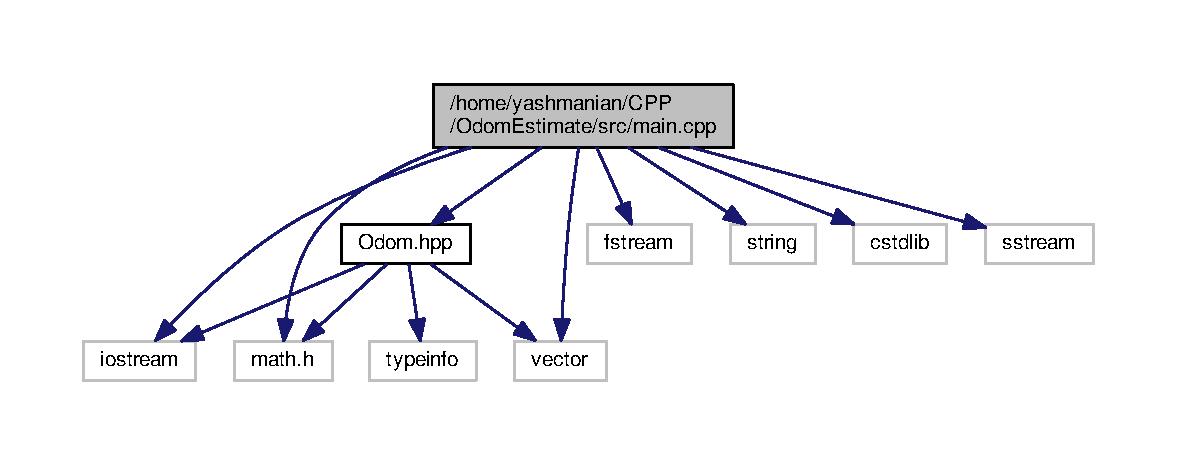
\includegraphics[width=350pt]{main_8cpp__incl}
\end{center}
\end{figure}
\subsection*{Macros}
\begin{DoxyCompactItemize}
\item 
\#define {\bfseries PI}~3.\+14159265358979323846\hypertarget{main_8cpp_a598a3330b3c21701223ee0ca14316eca}{}\label{main_8cpp_a598a3330b3c21701223ee0ca14316eca}

\end{DoxyCompactItemize}
\subsection*{Functions}
\begin{DoxyCompactItemize}
\item 
int \hyperlink{main_8cpp_ae66f6b31b5ad750f1fe042a706a4e3d4}{main} ()
\begin{DoxyCompactList}\small\item\em Function main that runs the main algorithm. \end{DoxyCompactList}\end{DoxyCompactItemize}


\subsection{Detailed Description}
Main function that brings it all together. 

M\+IT License Copyright (c) 2018 Yash Manian Permission is hereby granted, free of charge, to any person obtaining a copy of this software and associated documentation files (the \char`\"{}\+Software\char`\"{}), to deal in the Software without restriction, including without limitation the rights to use, copy, modify, merge, publish, distribute, sublicense, and/or sell copies of the Software, and to permit persons to whom the Software is furnished to do so, subject to the following conditions\+: The above copyright notice and this permission notice shall be included in all copies or substantial portions of the Software. T\+HE S\+O\+F\+T\+W\+A\+RE IS P\+R\+O\+V\+I\+D\+ED \char`\"{}\+A\+S I\+S\char`\"{}, W\+I\+T\+H\+O\+UT W\+A\+R\+R\+A\+N\+TY OF A\+NY K\+I\+ND, E\+X\+P\+R\+E\+SS OR I\+M\+P\+L\+I\+ED, I\+N\+C\+L\+U\+D\+I\+NG B\+UT N\+OT L\+I\+M\+I\+T\+ED TO T\+HE W\+A\+R\+R\+A\+N\+T\+I\+ES OF M\+E\+R\+C\+H\+A\+N\+T\+A\+B\+I\+L\+I\+TY, F\+I\+T\+N\+E\+SS F\+OR A P\+A\+R\+T\+I\+C\+U\+L\+AR P\+U\+R\+P\+O\+SE A\+ND N\+O\+N\+I\+N\+F\+R\+I\+N\+G\+E\+M\+E\+NT. IN NO E\+V\+E\+NT S\+H\+A\+LL T\+HE A\+U\+T\+H\+O\+RS OR C\+O\+P\+Y\+R\+I\+G\+HT H\+O\+L\+D\+E\+RS BE L\+I\+A\+B\+LE F\+OR A\+NY C\+L\+A\+IM, D\+A\+M\+A\+G\+ES OR O\+T\+H\+ER L\+I\+A\+B\+I\+L\+I\+TY, W\+H\+E\+T\+H\+ER IN AN A\+C\+T\+I\+ON OF C\+O\+N\+T\+R\+A\+CT, T\+O\+RT OR O\+T\+H\+E\+R\+W\+I\+SE, A\+R\+I\+S\+I\+NG F\+R\+OM, O\+UT OF OR IN C\+O\+N\+N\+E\+C\+T\+I\+ON W\+I\+TH T\+HE S\+O\+F\+T\+W\+A\+RE OR T\+HE U\+SE OR O\+T\+H\+ER D\+E\+A\+L\+I\+N\+GS IN T\+HE S\+O\+F\+T\+W\+A\+RE.

\begin{DoxyCopyright}{Copyright}
Copyright 2018 Yash Manian
\end{DoxyCopyright}
\begin{DoxyAuthor}{Author}
Yash Manian 
\end{DoxyAuthor}


\subsection{Function Documentation}
\index{main.\+cpp@{main.\+cpp}!main@{main}}
\index{main@{main}!main.\+cpp@{main.\+cpp}}
\subsubsection[{\texorpdfstring{main()}{main()}}]{\setlength{\rightskip}{0pt plus 5cm}int main (
\begin{DoxyParamCaption}
{}
\end{DoxyParamCaption}
)}\hypertarget{main_8cpp_ae66f6b31b5ad750f1fe042a706a4e3d4}{}\label{main_8cpp_ae66f6b31b5ad750f1fe042a706a4e3d4}


Function main that runs the main algorithm. 

Main function reads Encoder and time from a csv file. Parses file and passes values into a function. Saves the results in the Outputs folder. \begin{DoxyReturn}{Returns}
0 
\end{DoxyReturn}


Here is the call graph for this function\+:\nopagebreak
\begin{figure}[H]
\begin{center}
\leavevmode
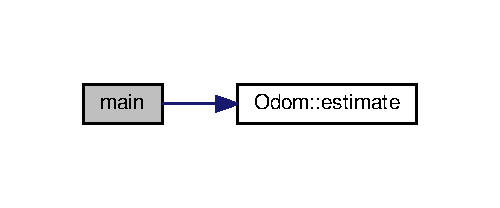
\includegraphics[width=240pt]{main_8cpp_ae66f6b31b5ad750f1fe042a706a4e3d4_cgraph}
\end{center}
\end{figure}



\hypertarget{_odom_8cpp}{}\section{/home/yashmanian/\+C\+P\+P/\+Odom\+Estimate/src/\+Odom.cpp File Reference}
\label{_odom_8cpp}\index{/home/yashmanian/\+C\+P\+P/\+Odom\+Estimate/src/\+Odom.\+cpp@{/home/yashmanian/\+C\+P\+P/\+Odom\+Estimate/src/\+Odom.\+cpp}}


Implementation of the methods of class \hyperlink{class_odom}{Odom}.  


{\ttfamily \#include \char`\"{}Odom.\+hpp\char`\"{}}\\*
Include dependency graph for Odom.\+cpp\+:\nopagebreak
\begin{figure}[H]
\begin{center}
\leavevmode
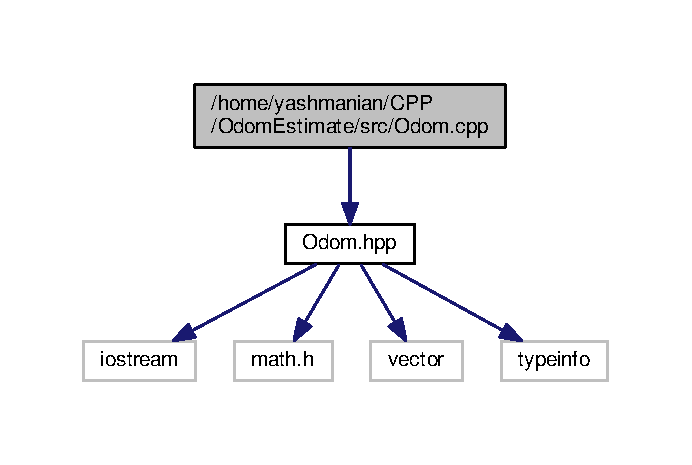
\includegraphics[width=332pt]{_odom_8cpp__incl}
\end{center}
\end{figure}


\subsection{Detailed Description}
Implementation of the methods of class \hyperlink{class_odom}{Odom}. 

M\+IT License Copyright (c) 2018 Yash Manian Permission is hereby granted, free of charge, to any person obtaining a copy of this software and associated documentation files (the \char`\"{}\+Software\char`\"{}), to deal in the Software without restriction, including without limitation the rights to use, copy, modify, merge, publish, distribute, sublicense, and/or sell copies of the Software, and to permit persons to whom the Software is furnished to do so, subject to the following conditions\+: The above copyright notice and this permission notice shall be included in all copies or substantial portions of the Software. T\+HE S\+O\+F\+T\+W\+A\+RE IS P\+R\+O\+V\+I\+D\+ED \char`\"{}\+A\+S I\+S\char`\"{}, W\+I\+T\+H\+O\+UT W\+A\+R\+R\+A\+N\+TY OF A\+NY K\+I\+ND, E\+X\+P\+R\+E\+SS OR I\+M\+P\+L\+I\+ED, I\+N\+C\+L\+U\+D\+I\+NG B\+UT N\+OT L\+I\+M\+I\+T\+ED TO T\+HE W\+A\+R\+R\+A\+N\+T\+I\+ES OF M\+E\+R\+C\+H\+A\+N\+T\+A\+B\+I\+L\+I\+TY, F\+I\+T\+N\+E\+SS F\+OR A P\+A\+R\+T\+I\+C\+U\+L\+AR P\+U\+R\+P\+O\+SE A\+ND N\+O\+N\+I\+N\+F\+R\+I\+N\+G\+E\+M\+E\+NT. IN NO E\+V\+E\+NT S\+H\+A\+LL T\+HE A\+U\+T\+H\+O\+RS OR C\+O\+P\+Y\+R\+I\+G\+HT H\+O\+L\+D\+E\+RS BE L\+I\+A\+B\+LE F\+OR A\+NY C\+L\+A\+IM, D\+A\+M\+A\+G\+ES OR O\+T\+H\+ER L\+I\+A\+B\+I\+L\+I\+TY, W\+H\+E\+T\+H\+ER IN AN A\+C\+T\+I\+ON OF C\+O\+N\+T\+R\+A\+CT, T\+O\+RT OR O\+T\+H\+E\+R\+W\+I\+SE, A\+R\+I\+S\+I\+NG F\+R\+OM, O\+UT OF OR IN C\+O\+N\+N\+E\+C\+T\+I\+ON W\+I\+TH T\+HE S\+O\+F\+T\+W\+A\+RE OR T\+HE U\+SE OR O\+T\+H\+ER D\+E\+A\+L\+I\+N\+GS IN T\+HE S\+O\+F\+T\+W\+A\+RE.

\begin{DoxyCopyright}{Copyright}
Copyright 2018 Yash Manian
\end{DoxyCopyright}
\begin{DoxyAuthor}{Author}
Yash Manian Estimates Pose and Odometry given Time, Angular Velocity, Encoder values and Steering Angle 
\end{DoxyAuthor}

%--- End generated contents ---

% Index
\backmatter
\newpage
\phantomsection
\clearemptydoublepage
\addcontentsline{toc}{chapter}{Index}
\printindex

\end{document}
